\section{Hipótese de Trabalho}

Ao integrar os resultados do LibScout ao contexto das ferramentas CryptoGuard e CogniCrypt, será possível não apenas detectar potenciais vulnerabilidades em APIs criptográficas, mas também identificar com precisão as correspondências associadas a bibliotecas externas, proporcionando uma abordagem mais abrangente e eficaz para a segurança de aplicações Java que utilizam operações criptográficas.

\section{Metodologia}

A metodologia abordada nestre trabalho serve como um instrumento complementar às metodologias e mecanismos descritas e abordadas no artigo 'Perceptions of Software Practitioners Regarding Crypto-API Misuses and Vulnerabilities'. \cite{perception_developers}
O trabalho realizado \cite{perception_developers} apresenta um estudo macro em relação à percepção das vulnerabilidades dos códigos dos desenvolvedores.

\begin{figure}[!h]
  \centering
  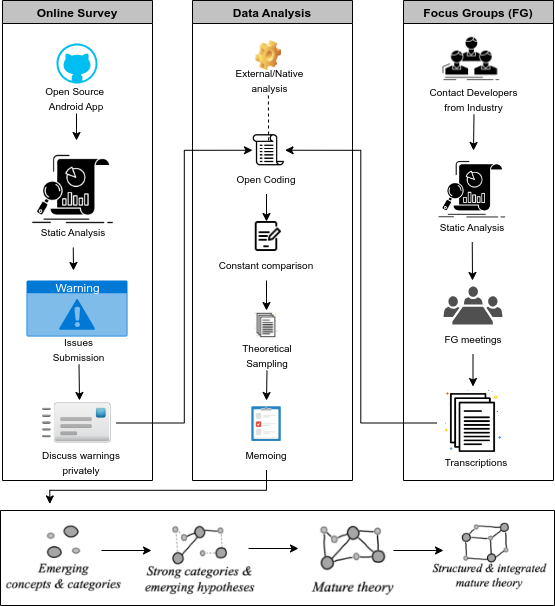
\includegraphics[scale=0.5]{img/metodologia.png}
  \caption{Metodologia adotada no artigo 'Perceptions of Software Practitioners Regarding Crypto-API Misuses and Vulnerabilities'}
  \label{averageWarnings}
\end{figure}


A imagem acima descreve a metodologia utilizada. \cite{perception_developers} A metodologia abordada neste trabalho entra na etapa de 'Análise de Dados' em específico 'Análise externa / nativa', onde é feita a integração dos resultados obtidos pelo LibScout com os contextos fornecidos pelo CryptoGuard e CogniCrypt. Essa integração tenta proporcionar uma visão mais minuciosa e contextualizada de onde as vulnerabilidades identificadas se encontram.
Este trabalho propõe a seguinte integração:

\begin{figure}[!h]
  \centering
  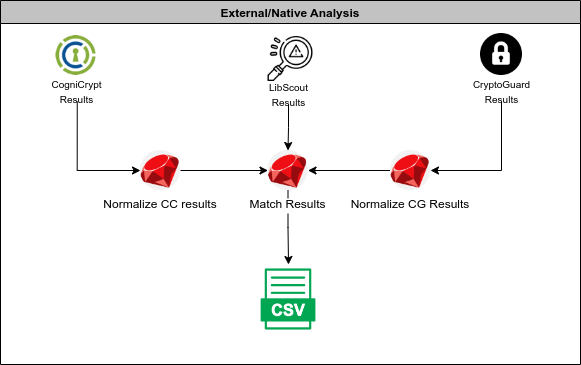
\includegraphics[scale=0.5]{img/studySettingsExternal.png}
  \caption{Metodologia adotada neste trabalho'}
  \label{averageWarnings}
\end{figure}

\begin{itemize}
\item{Coleta de Dados}
A metodologia adotada para a constituição do conjunto de dados envolveu uma cuidadosa seleção de aplicativos Java provenientes do renomado repositório F-Droid. \cite{perception_developers} Este último se destaca como um catálogo de aplicativos de código aberto e livre (FOSS), especialmente concebidos para a plataforma Android.

Nesse processo, buscou-se uma representativa diversidade de categorias de aplicativos, abrangendo áreas vitais como conectividade, finanças, segurança, mensagens de texto (SMS) e funcionalidades de sistema. Tal abordagem foi implementada com o intuito de assegurar uma abrangência abarcadora de contextos e finalidades, enriquecendo assim a robustez e representatividade do conjunto de dados analisado.

\item{Análise Estática}

A etapa subsequente consistiu na aplicação das ferramentas CryptoGuard e CogniCrypt para conduzir uma análise estática detalhada do código fonte dos aplicativos selecionados. Essa abordagem permitiu a identificação minuciosa de possíveis vulnerabilidades relacionadas às APIs criptográficas empregadas nos aplicativos avaliados. O uso dessas ferramentas especializadas proporcionou uma avaliação precisa e abrangente das práticas de segurança adotadas, visando aprimorar a integridade e robustez dos aplicativos em questão.

\item{Identificar a percepção de vulnerabilidade dos desenvoledores}

Após a conclusão da análise estática, foi possível identificar um conjunto de vulnerabilidades que não foram reconhecidas pelos desenvolvedores, bem como aquelas que foram identificadas, porém não receberam intervenção corretiva. Para facilitar a comunicação e o entendimento das questões de segurança identificadas, procedeu-se à criação de GISTS individuais para cada vulnerabilidade.  \cite{perception_developers}  Um GIST é um recurso que permite compartilhar trechos de código, arquivos inteiros ou até mesmo aplicações, e também possibilita a preservação e compartilhamento de saída de console ao executar, depurar ou testar o código. Cada GIST representa um repositório que pode ser clonado ou bifurcado por outras pessoas, promovendo assim a colaboração e a discussão ativa em busca do aprimoramento da segurança nos aplicativos avaliados.

\begin{figure}[!h]
  \centering
  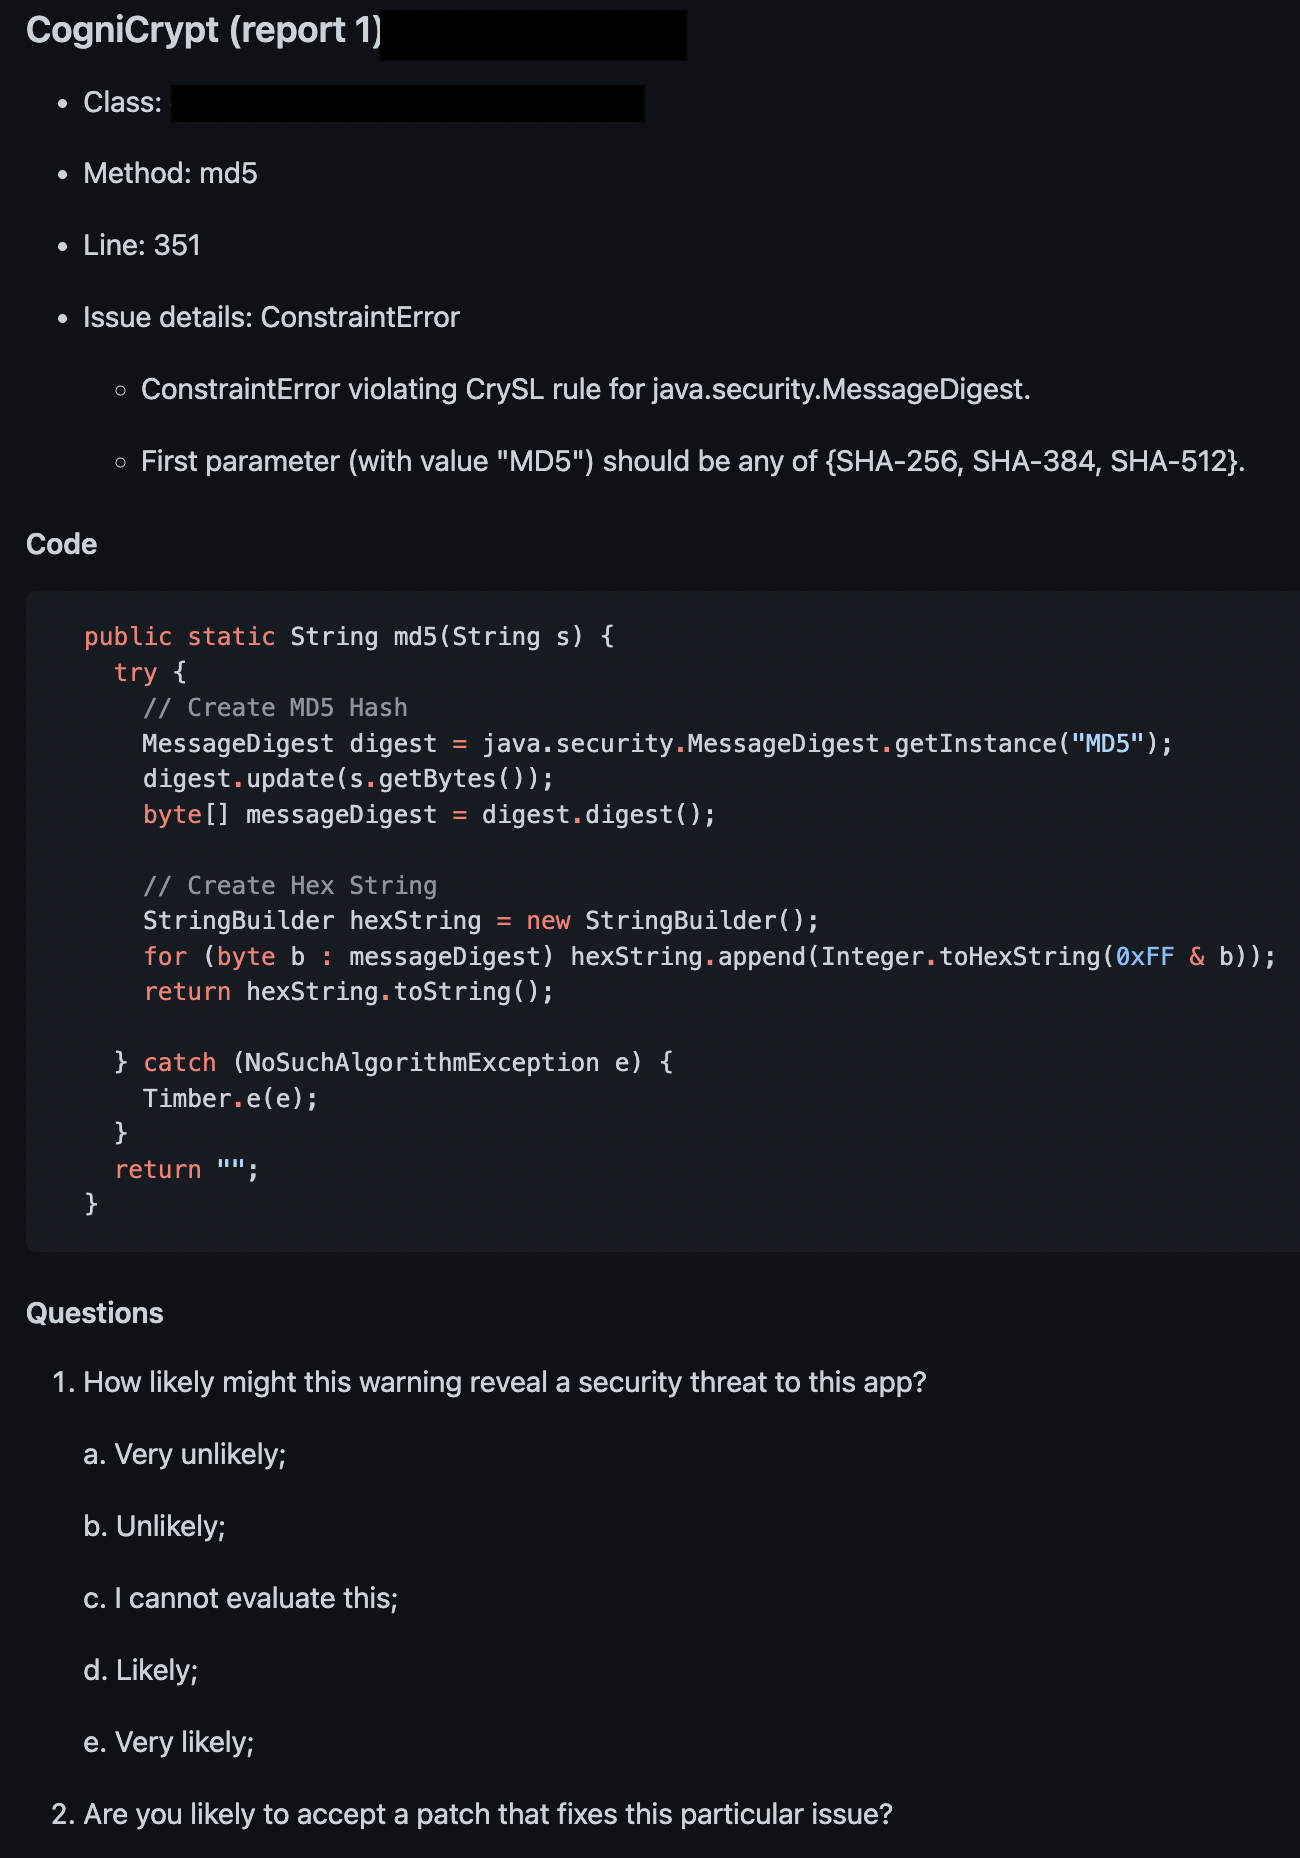
\includegraphics[scale=0.5]{img/gist.png}
  \caption{'Exemplo de uma Gist'}
  \label{averageWarnings}
\end{figure}

\item{Analisar origem das vulnerabilidades}

A etapa seguinte consistiu na análise da origem das vulnerabilidades identificadas. Para realizar essa análise, empregou-se a ferramenta LibScout, a qual desempenhou um papel crucial ao extrair informações detalhadas sobre as APIs criptográficas utilizadas nos aplicativos, permitindo, assim, a identificação de bibliotecas externas empregadas. A utilização do LibScout proporcionou um panorama abrangente das dependências externas dos aplicativos, fornecendo uma visão clara das fontes potenciais de vulnerabilidades no código. Esta abordagem foi essencial para direcionar os esforços na mitigação das ameaças identificadas e fortalecer a segurança das aplicações avaliadas.

A princípio, considerou-se a utilização do LibRadar devido à sua reputação pela rapidez de execução. Contudo, logo se constatou que a ferramenta estava baseada em dados disponibilizados até 2016, o que não condizia com nossa necessidade de informações atualizadas e abrangentes sobre as bibliotecas utilizadas nos aplicativos. Diante dessa constatação, optou-se por descartar o uso do LibRadar e buscar uma alternativa mais alinhada com os objetivos do estudo.

\item{Integração de Resultados}

Foi empreendido um esforço no sentido de desenvolver um processo de integração que possibilitasse a unificação dos resultados obtidos por meio do LibScout com os contextos fornecidos pelo CryptoGuard e CogniCrypt. Essa iniciativa tenta criar uma visão mais abrangente e contextualizada das vulnerabilidades identificadas. Em paralelo, foi realizada uma avaliação da eficácia dessa abordagem, no que tange à habilidade de determinar a origem dos alertas gerados pelas mencionadas ferramentas.

\end{itemize}

% Este capítulo oferece sugestões para produção de um documento descrevendo um Trabalho de Conclusão de curso...

% \section{UnB}%
% A \acrlong{UnB} oferece diversas informações em seu sítio\footnote{\url{http://www.unb.br/oportunidades/projeto_final_de_curso}}. O texto existente em 21/11/2014 é
% reproduzido a seguir:

% \fontshape{it}\selectfont%
% Os cursos de graduação, especialização e pós-graduação têm como objetivo formar o aluno e prepará-lo para o exercício profissional. Como avaliação do aprendizado, a universidade exige um projeto que mobiliza os estudantes a colaborar com a pesquisa acadêmica. Desde a escolha do tema até a apresentação do trabalho final, o tempo do aluno é ocupado quase integralmente. Para facilitar a vida desses estudantes, o Portal UnB preparou uma série de dicas de professores especialistas no assunto.

% \subsection{Os tipos}
% A monografia, a dissertação e a tese são, respectivamente, os trabalhos de conclusão de curso de graduação ou especialização, mestrado e doutorado. A grande diferença é a profundidade exigida no projeto, aumentada de acordo com a importância do título de cada nível acadêmico. Mas, em todos os casos, a pesquisa deve abordar o tema selecionado com coerência, consistência e referencial teórico adequado.

% Alguns cursos de graduação não exigem monografia, mas um relatório de estágios realizados, como acontece nas licenciaturas. A metodologia de pesquisar e apresentar resultados se mantém, como é exigido em todo projeto final.

% Uma monografia é, genericamente, um relatório de pesquisa sobre o assunto estudado. É específico a um tema pré-definido dentro de uma área de conhecimento e aborda questões e análises de um problema, a construção de uma teoria ou o desenvolvimento de um produto.

% Exigida no mestrado, a dissertação cobra do futuro mestre um conhecimento mais profundo. A pesquisa deve ser o resultado em relatório que representa o trabalho experimental ou exposição científica com um tema bem delimitado, e demonstrar o conhecimento de literatura existente sobre o assunto.

% A mais densa entre todos os projetos finais, a tese de doutorado exige mais no que diz respeito a teoria e metodologia do tema pesquisado. Deve apresentar contribuições reais para o desenvolvimento específico da especialidade em questão. A base do estudo demanda uma investigação original.

% \subsection{Teoria e prática}
% Todo projeto de conclusão de curso exige um relatório escrito baseado em teorias, mesmo que o assunto estudado seja algo prático como uma campanha publicitária ou um projeto arquitetônico. Porém, o inverso não se aplica.

% As divisões dos tipos de trabalho variam entre cada área de conhecimento. Em suma, o projeto pode ser teórico, prático ou uma união dos dois. Na primeira situação, o aluno pode fazer estudo de caso - pesquisar sobre um fato histórico ou evento importante - ou formular uma teoria - por meio de pesquisa ou reavaliação das semelhantes.

% O projeto prático se dedica a criação e construção de um produto, que pode variar de um novo motor a uma composição musical. O curso de graduação costuma oferecer a opção de um trabalho prático aos alunos. No caso dos cursos de mestrado e doutorado, nem todos os departamentos da universidade dispõem de linhas de pesquisa que permitam um projeto que vá além da teoria acadêmica.

% A união dos dois gêneros é comum quando o universitário relata a experiência de estágio ou na simulação de um projeto, como a construção de maquetes ou esquemas computacionais. As opções são vastas e o aluno deve explicar como e o que se deve fazer para que o projeto se torne possível.

% \subsection{Começo do projeto}
% Parece óbvio, mas muitos alunos esquecem a questão principal na hora de escolher o tema: o assunto deve interessar e estimular a pesquisa. Conviver meses com um tema que não agrada torna o trabalho mais complicado. Porém, escolher um bom tema não é abraçar e desenvolver sobre tudo que ele é e engloba. É preciso delimitar o assunto de forma específica.

% Um trabalho sobre a história do mundo, por exemplo, está fadado a se tornar superficial. Além de extremamente amplo, é grande o volume de informações a ser levantado e estudado. É importante ter foco para desenvolver um projeto coeso e com credibilidade.

% Além disso, o estudante necessita desenvolver um problema e traçar uma hipótese. Em um exemplo bem simples: a Guerra no Iraque (tema) e o terrorismo mundial (problema) – o aumento dos ataques depois da invasão americana (hipótese); ou seja, o que o aluno quer tratar e onde ele espera chegar na pesquisa. A não comprovação da hipótese não inviabiliza o trabalho, desde que o desenvolvimento da análise enriqueça os conhecimentos sobre o tema tratado.

% A prática essencial para o desenvolvimento de qualquer projeto é a pesquisa bibliográfica. As consultas às bibliotecas respaldam a parte teórica do estudo e podem elucidar diversas questões, sejam específicas do projeto ou sobre metodologias científicas. Nesse ponto, o papel do professor orientador é fundamental para a condução da pesquisa. Além da seleção dos livros, o docente analisa as melhores possibilidades de desenvolver o assunto, em todas as suas fases. Ele também pode indicar a aplicação de entrevistas e outros elementos de apoio ao conteúdo do projeto.

% Atualmente, o meio mais difundido de pesquisa é a Internet. Além de facilitar o acesso a documentos, pela rede é possível saber quanto o tema escolhido já foi objeto de estudo de outros acadêmicos. Mas essa facilidade deve ser utilizada para indicar um caminho.

% \subsection{Estrutura e regras}
% Antes do próprio trabalho escrito, o estudante deve fazer um projeto ou plano de pesquisa. O documento identifica o que deve ser feito, o porquê, como e onde será realizado o levantamento. Não há um modelo rígido para a apresentação do projeto de pesquisa, mas os seguintes elementos devem ser respondidos no texto:

% \begin{enumerate}
%   \item Definição do objeto de estudo (tema/problema da pesquisa)
%   \item Justificativa
%   \item Hipóteses de trabalho
%   \item Discussão teórica
%   \item Metodologia
%   \item Pesquisa Bibliográfica
% \end{enumerate}

% Seja monografia, dissertação ou tese, a parte escrita possui uma estrutura semelhante, embora cada uma tenha características próprias referentes à profundidade do tema estudado.

% De acordo com a Associação Brasileira de Normas Técnicas (ABNT), um trabalho acadêmico deve englobar os elementos pré-textuais (como resumo e índice), pós-textuais (bibliografia, anexos, entre outros) e textuais. Esses últimos compõem a parte central do trabalho - introdução, desenvolvimento e conclusão.

% A introdução é a parte inicial do texto e deve constar o objeto de pesquisa, os objetivos, a justificativa da escolha do tema e outras informações que sejam necessárias para esclarecer o assunto.

% A parte principal do trabalho está concentrada no desenvolvimento. É uma exposição sistematizada e ordenada de toda o estudo desenvolvido, apresentando análise e interpretação das informações e dados obtidos. A conclusão é a etapa final do texto. Nela, são apresentados os resultados tendo como referência os objetivos e hipóteses da pesquisa.

% Em todo o trabalho a linguagem utilizada deve ser interessante, sem apelar para a linguagem coloquial. O trabalho deve estar de acordo com as normas da ABNT. Procure livros sobre estrutura e regras do tipo de projeto final específico de seu interesse.

% \subsection{O projeto está pronto. E agora?}
% Após a finalização do projeto, chega o momento de preparar a apresentação. Em geral, a banca examinadora é formada por três docentes, sendo um deles o professor orientador do projeto. Também é comum aos alunos o direito de escolha dos avaliadores, desde que seja pertinente ao assunto e ao objetivo do estudo.

% Esses professores recomendam uma apresentação resumida do projeto, pontuando as características essenciais e como se chegou às conclusões. É sempre bom explicar o cronograma de todo o trabalho. É preciso, também, ficar atento ao tempo. Não é necessário explicar os conceitos já citados no projeto e pode influenciar a nota final. Lembre-se que as explicações são voltadas para os avaliadores, que já leram o seu trabalho.

% Durante as considerações da banca examinadora não se deve interromper a avaliação dos professores, exceto quando eles dirigirem diretamente uma pergunta ao aluno. Educação e conhecimento dos procedimentos acadêmicos são essenciais para uma boa apresentação. Após a avaliação, os professores pedem para os presentes se retirarem da sala. É feita uma reunião onde será decidida a nota do projeto.

% Cada departamento possui regras e orientações para a apresentação dos trabalhos de conclusão. Cabe ao aluno perguntar à coordenação do curso e ao orientador todas as etapas do processo de elaboração do projeto final.

% \fontshape{n}\selectfont%
